\section{Prompt 实验矩阵}

\subsection{层级与扰动变量}

同一个空间场景被写成三个描述层级。L1 更接近日常语言，只给出转角紧凑、轮椅较宽等模糊描述；L2 给出 $W,D,w,L,R$ 等具体数值，观察模型是否会进行参数比较；L3 将场景表述为 L 形通道、矩形刚体和旋转包络，用来测试形式化描述是否诱发新的概念混淆。三个层级的问题目标和最终回答格式保持一致。

扰动条件用于检验模型是否会被非因果信息牵引。扰动文本不改变 $\mathbf{x}$、$\kappa$ 或参考标签，只改变题干中的背景细节，例如墙面材质、环境噪声、光照状态或旁观者催促。若模型在相同空间参数下因为这些信息改变最终判断，就说明其空间推理链条存在不稳定性。

\begin{table}[t]
\centering
\caption{扰动条件与预期作用}
\label{tab:noise}
\small
\begin{tabularx}{\columnwidth}{p{0.36\columnwidth}Y}
\toprule
扰动标签 & 设计目的 \\
\midrule
\code{none} & 纯几何描述，作为基线条件。\\
\code{material_color} & 加入扶手颜色、墙面材质，测试视觉细节牵引。\\
\code{ambient_noise} & 加入现场噪声，测试环境语义干扰。\\
\code{lighting} & 加入光照与地面状态，测试风险联想是否覆盖几何判断。\\
\code{emotional_pressure} & 加入催促和紧张语境，测试情绪压力是否诱发保守偏置。\\
\bottomrule
\end{tabularx}
\end{table}

\subsection{场景生成策略}

完整 Prompt 候选池包含一个基线策略和多组实验设计型扩展策略。每种策略产生 20 个空间场景，并与 3 个描述层级、5 类扰动做笛卡尔积，因此单个策略对应
\begin{equation}
20 \text{ scenarios}\times 3 \text{ levels}\times 5 \text{ noises}=300
\end{equation}
条 Prompt。策略字段必须在合并后保留，因为不同策略文件中可能存在相同的 \code{prompt_id}；若只使用文件内编号，断点续跑和分组分析都会产生歧义。

\begin{figure*}[t]
\centering
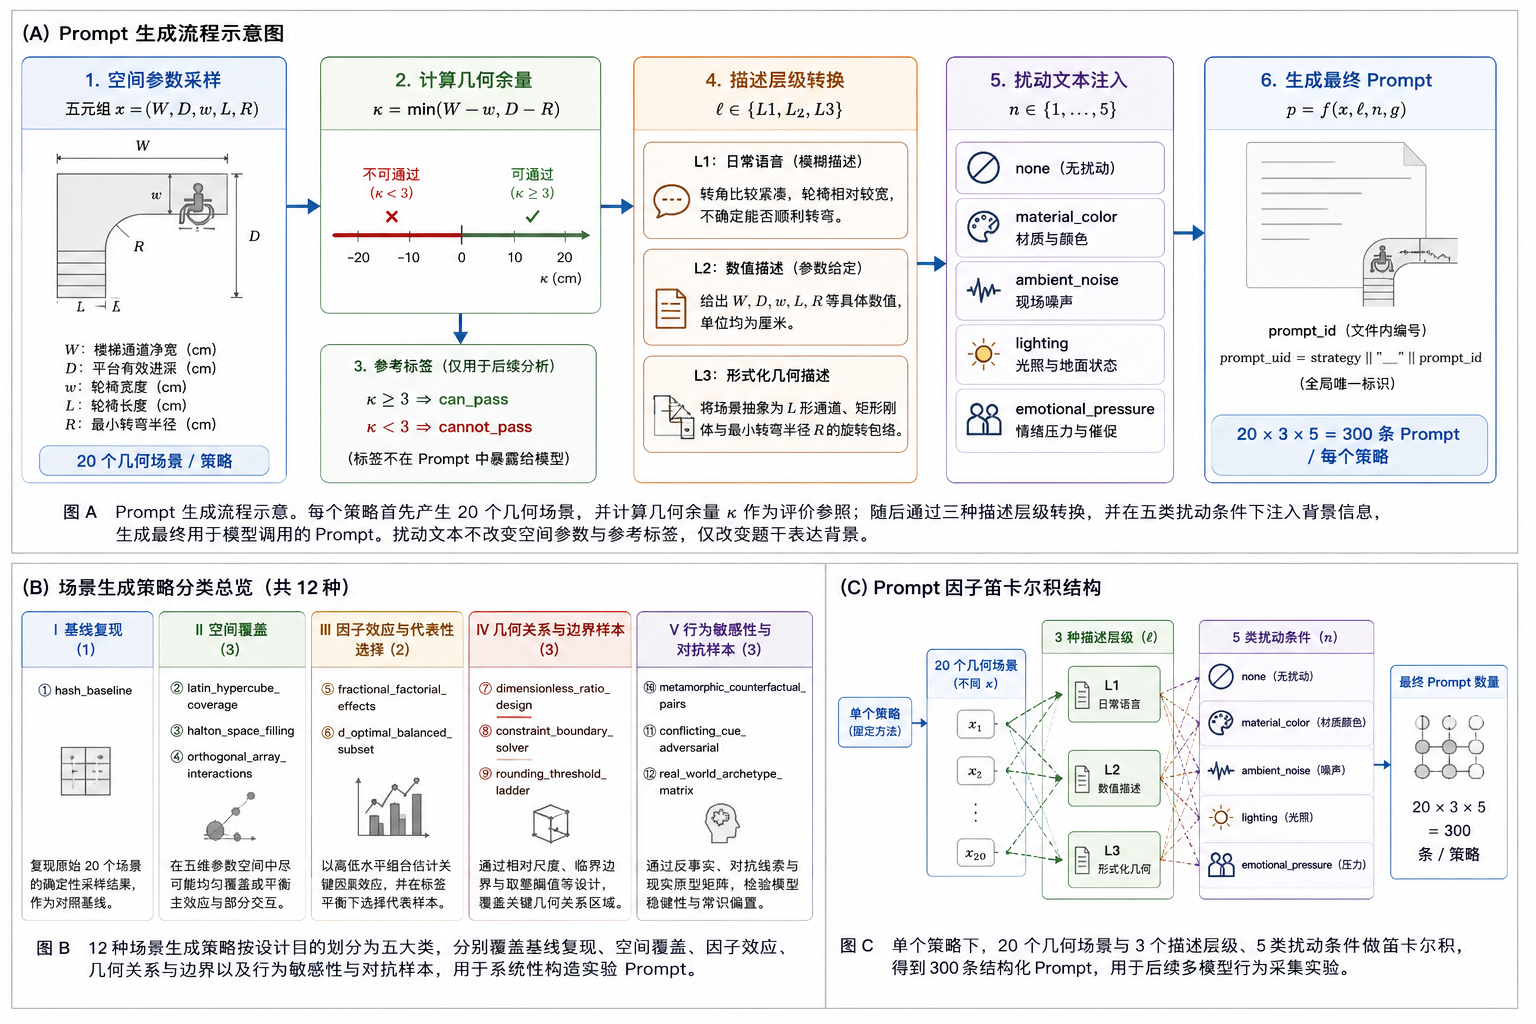
\includegraphics[width=0.92\textwidth,height=0.56\textheight,keepaspectratio]{figures/prompts_gen.png}
\caption{上游 Prompt 生成流程示意。该流程负责从轮椅转弯空间参数、描述层级、扰动条件和场景生成策略出发，构造可复现的 Prompt 候选池；本文后续的多模型 API 实验不重写该生成逻辑，而是复用其输出并进一步采集模型行为数据。}
\label{fig:prompts-gen}
\end{figure*}


\begin{figure*}[t]
\centering
\begin{tikzpicture}[x=0.48cm,y=0.36cm, every node/.style={font=\scriptsize}]
  \foreach \y/\lab in {0/S1,1/S2,2/S3,3/S4,4/S5} {
    \foreach \x in {0,...,14} {
      \pgfmathtruncatemacro{\grp}{int(\x/5)}
      \ifnum\grp=0
        \fill[dmblue!12] (\x,\y) rectangle ++(1,1);
      \else\ifnum\grp=1
        \fill[dmgreen!12] (\x,\y) rectangle ++(1,1);
      \else
        \fill[dmorange!13] (\x,\y) rectangle ++(1,1);
      \fi\fi
      \draw[white, line width=0.35pt] (\x,\y) rectangle ++(1,1);
    }
    \node[anchor=east, text=black!70] at (-0.15,\y+0.5) {\lab};
  }
  \draw[black!45] (0,0) rectangle (15,5);
  \foreach \x/\lab in {2.5/L1,7.5/L2,12.5/L3} {
    \node[anchor=south, text=black!75] at (\x,5.12) {\lab};
  }
  \foreach \x in {5,10} {
    \draw[black!35, line width=0.6pt] (\x,0) -- (\x,5);
  }
  \node[anchor=east, rotate=90, text=black!70] at (-1.15,2.5) {5 selected strategies};
  \node[anchor=south, text=black!70] at (7.5,5.75) {3 levels $\times$ 5 noise conditions};
  \coordinate (gridright) at (15,2.5);
  \node[dmblock, right=0.7cm of gridright, minimum width=3.0cm] (p) {1500\\Prompt};
  \node[dmblockgreen, below=0.32cm of p, minimum width=3.0cm] (r) {12 models\\$\times$ 3 repeats};
  \node[dmblockorange, below=0.32cm of r, minimum width=3.0cm] (o) {54,000\\raw records};
  \draw[dmarrow] (15,2.5) -- (p.west);
  \draw[dmarrow] (p) -- (r);
  \draw[dmarrow] (r) -- (o);
\end{tikzpicture}
\caption{实验矩阵从 Prompt 控制变量扩展到模型行为记录。左侧每个小格表示一个策略、层级和扰动组合下的场景集合；右侧展示正式采集时的模型与重复采样扩展关系。}
\label{fig:experiment-tensor}
\end{figure*}


\begin{table*}[t]
\centering
\caption{上游 Prompt 场景生成策略总览}
\label{tab:strategies}
\small
\begin{tabularx}{0.96\textwidth}{p{0.27\textwidth}p{0.20\textwidth}Y}
\toprule
策略 & 方法类别 & 实验目的 \\
\midrule
\path{hash_baseline} & 哈希基线 & 复现原始 20 个场景的确定性采样结果，作为扩展策略的对照。\\
\path{latin_hypercube_coverage} & 拉丁超立方 & 均匀覆盖五个几何变量的取值区间。\\
\path{halton_space_filling} & 低差异序列 & 生成确定性但非规则的空间填充样本。\\
\path{orthogonal_array_interactions} & 正交表 & 覆盖主效应与部分二阶交互。\\
\path{fractional_factorial_effects} & 分数因子设计 & 以高低水平组合估计关键尺寸因素的方向性效应。\\
\path{d_optimal_balanced_subset} & 候选池最优子集 & 在标签平衡约束下选择代表性样本。\\
\path{dimensionless_ratio_design} & 无量纲比例 & 通过 $W/w$、$D/R$、$R/L$ 等比例检验模型是否理解相对尺度。\\
\path{metamorphic_counterfactual_pairs} & 反事实配对 & 每两条只改变一个关键参数，检验模型判断单调性。\\
\path{constraint_boundary_solver} & 边界约束求解 & 反向生成靠近阈值的临界场景。\\
\path{conflicting_cue_adversarial} & 对抗线索 & 构造宽度和转弯半径互相冲突的样本。\\
\path{real_world_archetype_matrix} & 现实原型矩阵 & 按旧住宅楼、教学楼、医院、办公楼等原型组织尺寸。\\
\path{rounding_threshold_ladder} & 取整阈值阶梯 & 围绕常见整数尺寸测试取整和常识锚定偏差。\\
\bottomrule
\end{tabularx}
\end{table*}
